%!TEX root = hems_proj.tex
%%%%%%%%%%%%%%%%%%%%%%%%%%%%%%%%%%%%%%%%%%%%%%%%%%%%%%%%%%%%%%%%%%%%%%%
\chapter{Következtetések és Ajánlások}\label{ch:ELEMZES}

\section{Egy nap részletes esetelemzése}
A \ref{fig:winter_day}. ábra a téli szcenárió egy tipikus napjának PV-termelés és fogyasztási profiljait mutatja. A \ref{tab:winter_stats}. táblázat eredményei alapján ebben a körülményben a GWO adta a legalacsonyabb átlagos költséget, ami összhangban van a szűkös termelési helyzettel.

\begin{figure}[H]
\centering
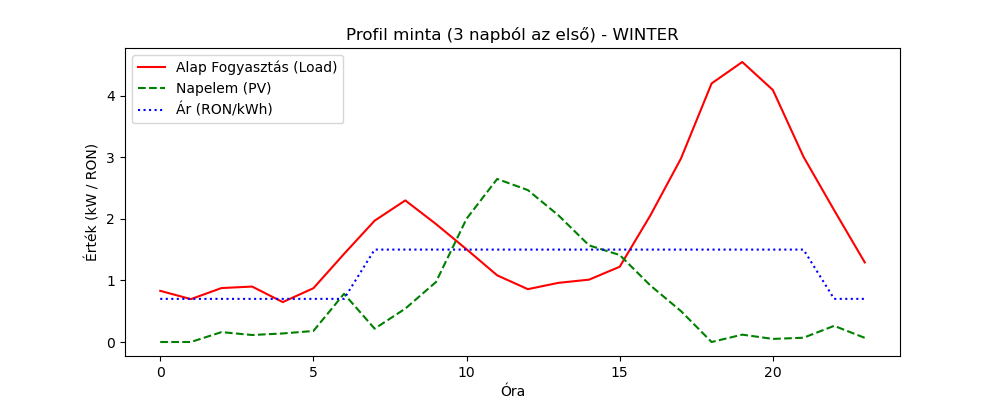
\includegraphics[width=0.85\textwidth]{ekim2339_proj/generated_day_winter.png}
\caption{Téli bemeneti profilok (PV termelés és fogyasztás)}
\label{fig:winter_day}
\end{figure}

\begin{figure}[H]
\centering
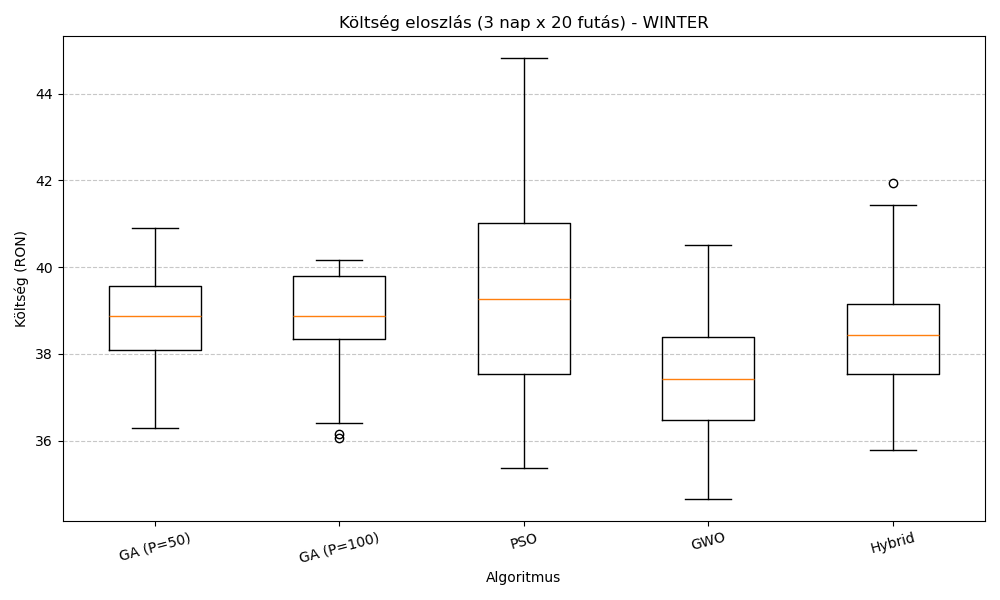
\includegraphics[width=0.85\textwidth]{ekim2339_proj/results_boxplot_winter.png}
\caption{Költség eloszlás a téli szcenárióban (20 futás)}
\label{fig:winter_box}
\end{figure}

\section{Főbb megállapítások}
A kísérletek rávilágítottak a \textbf{szezonális különbségek} fontosságára. Nyáron az optimalizáció kulcsa a többlettermelés menedzselése (az akkumulátor töltése vagy visszatáplálás), míg télen a drága csúcsidőszaki fogyasztás minimalizálása a cél. A vizsgált három szcenárió (tél, nyár, borús) megfelelően lefedi a valós üzemeltetési körülményeket. Az \textbf{algoritmus választást} illetően megállapítható, hogy nincs egyetlen "legjobb" módszer. A GA (P=100) a komplex, változékony esetekben bizonyult robusztusnak, míg a GWO a szigorúbb korlátokkal terhelt téli környezetben működött hatékonyabban. Az \textbf{akkumulátor szerepe} különösen a borús tesztesetben mutatkozott meg, ahol kulcsfontosságúnak bizonyult a termelés ingadozásainak kisimításában. A \textbf{futási teljesítmény} tekintetében az algoritmusok 0.21 és 0.92 másodperc közötti idő alatt találtak megoldást; a PSO volt a leggyorsabb, de ez gyakran a megoldás minőségének rovására ment.

\section{Gazdasági megtérülés}
\begin{table}[H]
\centering
\caption{Beruházási és megtérülési kalkuláció becslés}
\begin{tabular}{lc}
\toprule
\textbf{Tétel} & \textbf{Költség/Érték} \\
\midrule
HEMS hardver & $\approx$ 1200 RON \\
5 kWp napelem rendszer & $\approx$ 15000 RON \\
10 kWh akkumulátor & $\approx$ 18000 RON \\
\midrule
\textbf{Teljes beruházás} & \textbf{$\approx$ 34200 RON} \\
\midrule
Éves megtakarítás (becsült) & $\approx$ 6200 RON \\
\midrule
\rowcolor{yellow!30}
\textbf{Megtérülési idő} & \textbf{$\approx$ 5.5 év} \\
\bottomrule
\end{tabular}
\end{table}
Támogatással (Casa Verde) a megtérülés 3--4 évre csökkenthető.

\section{Környezeti hatás}
A rendszer környezeti hatása jelentős. Az évi 6000 kWh saját napelemes termelés önmagában mintegy 4.8 tonna CO$_2$ kiváltását eredményezi. Ehhez adódik hozzá a terhelés-eltolásból és a hatékonyságnövelésből származó további 2000 kWh megtakarítás, ami újabb 1.6 tonna kibocsátáscsökkenést jelent. \textcolor{red}{\textbf{Összességében így évente nagyságrendileg 6.4 tonna CO$_2$ megtakarítás érhető el.}}

\section{Jövőbeli kutatási irányok}
\subsection{Energiaközösségek (REC)}
Peer-to-peer energia kereskedés, közösségi akkumulátor; potenciális további megtakarítás 10--15\%.

\subsection{Multi-objective optimalizálás}
Pareto-front alapú megközelítés: felhasználó választhat költség-komfort görbéről, adaptív súlyozással.

\subsection{Gépi tanulás integráció}
LSTM időjárás előrejelzés, felhasználói szokások tanulása, prediktív karbantartás.

\subsection{V2G integráció}
Elektromos autók mint mobil akkumulátorok: 60 kWh EV kapacitás $\rightarrow$ 6x nagyobb tárolás, 50--100 RON/hó extra bevétel.

\section{Implementációs ajánlások}
\subsection{Kis háztartásoknak (< 3 fő)}
\textbf{Kis háztartásoknak} egy minimális konfiguráció javasolt, amely egy HEMS vezérlőből és intelligens konnektorokból áll. Ennek beruházási költsége alacsony, 800--1200 RON közé tehető. A rendszerrel elérhető 15--20\%-os megtakarítás (évi 500--800 RON) mellett a befektetés várhatóan 1.5--2 év alatt megtérül.

\subsection{Közepes háztartásoknak (3--5 fő)}
\textbf{Közepes háztartásoknak} egy komolyabb rendszer kiépítése ajánlott, amely a HEMS mellett egy 3--5 kWp-es napelemes rendszert és egy 5--10 kWh kapacitású akkumulátort is tartalmaz. Bár a beruházás összege 25000--35000 RON, ez támogatásokkal csökkenthető. A várható megtakarítás ebben az esetben jelentős, 30--50\% (évi 3000--5000 RON), így a megtérülési idő támogatással 3--5 évre, támogatás nélkül 6--8 évre becsülhető.
